\documentclass[a4paper,12pt]{article}
\usepackage[utf8]{inputenc}
\usepackage[spanish]{babel}
\usepackage{color}
\usepackage{parskip}
\usepackage{graphicx}
\usepackage{multirow}
\usepackage{listings}
\usepackage{vmargin}
\usepackage{datetime}
\usepackage{float}
\newdate{date}{24}{08}{2017}
\graphicspath{ {imagenes/} }
\definecolor{mygreen}{rgb}{0,0.6,0}
\definecolor{lbcolor}{rgb}{0.9,0.9,0.9}
\usepackage{epstopdf}


\setpapersize{A4}
\setmargins{2.5cm}       % margen izquierdo
{1.5cm}                        % margen superior
{16.5cm}                      % anchura del texto
{23.42cm}                    % altura del texto
{10pt}                           % altura de los encabezados
{1cm}                           % espacio entre el texto y los encabezados
{0pt}                             % altura del pie de página
{2cm}     

\lstset{
backgroundcolor=\color{lbcolor},
    tabsize=4,    
%   rulecolor=,
    language=[GNU]C++,
        basicstyle=\tiny,
        aboveskip={1.5\baselineskip},
        columns=fixed,
        showstringspaces=false,
        extendedchars=false,
        breaklines=true,
        prebreak = \raisebox{0ex}[0ex][0ex]{\ensuremath{\hookleftarrow}},
        frame=single,
        showtabs=false,
        showspaces=false,
        showstringspaces=false,
        identifierstyle=\ttfamily,
        keywordstyle=\color[rgb]{0,0,1},
        commentstyle=\color[rgb]{0.026,0.112,0.095},
        stringstyle=\color{red},
        numberstyle=\color[rgb]{0.205, 0.142, 0.73},
%        \lstdefinestyle{C++}{language=C++,style=numbers}’.
}


\begin{document}
\title{Cuestionario Previo de la Primera Práctica}
\author{
Christofer Fabián Chávez Carazas \\
\small{Universidad Nacional de San Agustín de Arequipa} \\
\small{Escuela Profesional de Ciencia de la Computación} \\
\small{Computación entrada en Redes}
}
\date{\displaydate{date}}

\maketitle

\begin{enumerate}
 {\large \item  \textbf{Describa el puerto serie}} \par
  Un puerto serial es una interfaz de computadora que transmite datos
  un bit a la vez \cite{serialbook}, siendo este la principal desventaja frente a los
  puertos en paralelo.
  Comúnmente, el término ``puerto serial'' se refiere al puerto
  que usa un protocolo asíncrono en particular, que en muchos de los casos
  son de comunicación bidireccional; los puertos envían y reciben datos a la vez. \\
  Existen varios estándares para poder armar una comunicación serial.
 
  {\large \textbf{Estándar RS-232}} \\
  RS-232 es el estándar más usado para la comunicación serial. 
  Fue estandarizado en 1962 por \textit{Electronics Industries Association} (EIA).
  Lamentablemente el estándar sólo permite una distancia máxima de enlace de 15 metros y
  una velocidad de transmisión de máximo 20 Kbps \cite{serialstandars}. \\
  El estándar nos dice que usemos el conector de 25 pines. En la Figura \ref{fig:db25}
  se muestra un conector DB25S con algunos de los pines que se utilizan.
  
  \begin{figure}
   \centering
   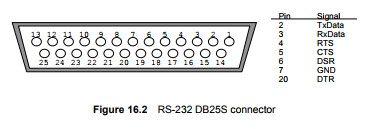
\includegraphics[scale = 0.6]{2.png}
   \caption{Interfaz RS-232 DB25S \cite{rs232}}
   \label{fig:db25}
  \end{figure}
  
  Aunque este es el conector que el estándar nos dice que usemos, actualmente
  se utiliza otro tipo de conector con menos pines, ya que no es indispensable
  usar los 25 pines para establecer una comunicación entre dos equipos. Por esta razón
  se utiliza conectores de 9 pines. En la Figura \ref{fig:db9} se muestra un conector
  DB9S con los pines utilizados. Los tipos de señales especificados en el estándar
  son los siguientes \cite{serialstandars}:
  \begin{itemize}
   \item \textbf{Masa:} GND para aislamiento del conector con enlace al chasis de la terminal; SG Señal sobre la que se establece la tensión de las demás señales del conector
   \item \textbf{Canal Principal:} Conjunto de señales de datos y control, TxD y RxD líneas de transmisión y recepción 
   respectivamente; RTS, CTS, DSR y DCD señales básicas, DTR y RI señales conmutadas y SQ, CH y CI señales de calidad y canales.
   \item \textbf{Transmisión Síncrona:}  DA, DD y DB exclusivas de sincronía.
   \item \textbf{Canal Secundario:} para algunos modelos DCE.
   \item \textbf{Terminales sin Asignación Fija.}
  \end{itemize}

  \begin{figure}
   \centering
   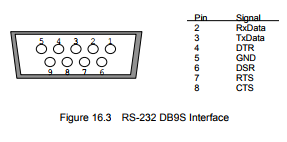
\includegraphics[scale = 0.6]{1.png}
   \caption{Interfaz RS-232 DB9S \cite{rs232}}
   \label{fig:db9}
  \end{figure}
  
  El estándar también define características para la parte eléctrica. La norma define
  un margen de tensión de +3 V a +25 V para el ``0'' lógico y -3 V a -25 V para el ``1'' lógico \cite{rs232}. \par
  
  RS-232 usa comunicación asíncrona, como se mencionó anteriormente, que tiene un formato de datos
  \textit{stat-stop}. Cada caracter es transmitido uno a la vez con un pequeño tiempo entre ellos.
  Este tiempo es llamado inactivo. El transmisor envía el bit de inicio para informar al receptor
  que un caracter está siendo enviado. Este bit de inicio suele ser ``0''. Luego se envía hasta un máximo
  de 7 bits como un \textit{7-bit ASCII character}, seguido de un bit de paridad y, finalmente, 1, 1.5 o 2 bits de pare.
 
  
 {\large \item  \textbf{Describe el puerto paralelo}} \par
 Al igual que un puerto serial, un puerto paralelo es una interfaz de computadora que nos
 permite entablar una comunicación, pero con la diferencia de que los puertos paralelos
 pueden transmitir múltiples bits al mismo tiempo \cite{parallelbook}. \\
 
 {\large \textbf{SPP}} \\
 El SPP o \textit{Standard Parallel Port} es el puerto original de la IBM PC y vendría
 a ser, como su nombre lo dice, es un estándar antiguo dentro de los puertos paralelos. El puerto
 original estuvo basado en la interfaz Centronics para impresoras. \\
 
 {\large \textbf{IEEE 1284}}\\ 
 La IEEE 1284 es un estándar más nuevo para la transmisión en paralelo \cite{IEEEparallel}.
 Este estándar define varios modos para un puerto paralelo:
 \begin{itemize}
  \item \textbf{Modo de Compatibilidad:} Básicamente en este modo se mueven datos desde una PC hacia
  un periférico como una impresora. Se pueden mover hasta 8 bits de datos al mismo tiempo.
  \item \textbf{Modo Nibble:} Es lo contrario al modo anterior; se mueven datos desde el periférico hacia la PC.
  Se pueden mover hasta un nibble de información (4 bits).
  \item \textbf{Modo Byte:} Es igual que el modo nibble solo que ahora se puede mover
  hasta un byte de información.
  \item \textbf{Modo EPP:} Este modo funciona de forma bidireccional.
 \end{itemize}

 Al igual que en los puertos seriales, este estándar define la velocidad máxima que puede alcanzar
 un puerto paralelo. Dependiendo del puerto que se utilice, este puede alcanzar una velocidad de hasta 
 150 Kbps, 1.5 Mbps y 2.5 Mbps. El estándar nos ofrece alternativas en los conectores.
 El tradicional tipo D de 25 pines es llamado IEEE 1284-A (Figura \ref{fig:IEEE1}), el tradicional conector
 \textit{Centronics} es llamado IEEE 1284-B (Figura \ref{fig:IEEE2}), y un nuevo conector más pequeño similar al conector \textit{Centronics}
 es llamado IEEE 1284-C (Figura \ref{fig:IEEE3}).
 
 
 \begin{figure}
   \centering
   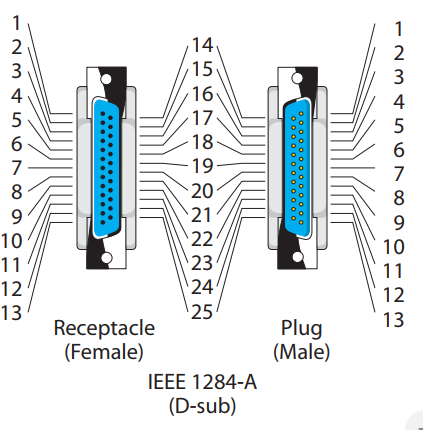
\includegraphics[scale = 0.4]{3.png}
   \caption{Conector IEEE 1284-A \cite{IEEEparallel}}
   \label{fig:IEEE1}
  \end{figure}
  
  \begin{figure}
   \centering
   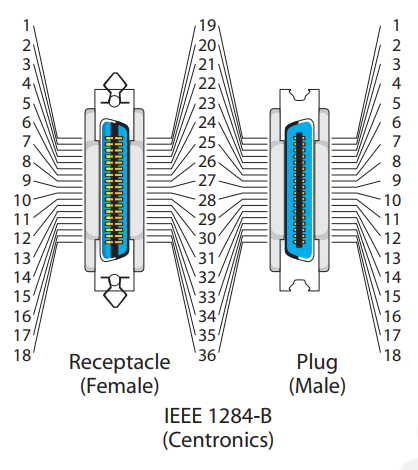
\includegraphics[scale = 0.4]{4.png}
   \caption{Conector IEEE 1284-B \cite{IEEEparallel}}
   \label{fig:IEEE2}
  \end{figure}
  
  \begin{figure}
   \centering
   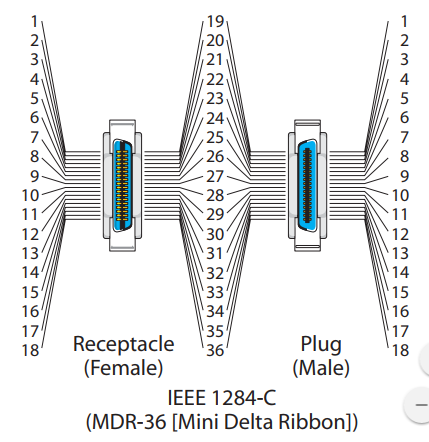
\includegraphics[scale = 0.4]{5.png}
   \caption{Conector IEEE 1284-C \cite{IEEEparallel}}
   \label{fig:IEEE3}
  \end{figure}
 
 \newpage
 
 {\large \item \textbf{Describe el puerto usb}} \par
 El USB (\textit{Universal Serial Bus}) es el estándar actual de la comunicación serial. \cite{usb}. El estándar define la velocidad máxima de una comunicación
 usb en 12 Mbps. Para evitar que el usuario genere problemas con los conectores, USB utiliza el protocolo \textit{keyed connector}. En la Figura
 \ref{fig:usb} se muestran los diferentes tipos de conectores USB que existe. Las diferencias físicas entre los conectores se debe a la conectividad que tiene el usuario.
 El conector de serie A es principalmente para conectar dispositivos USB directamente al host. Los conectores de serie B y mini-B
 están pensados para ser usados mediante un cable desechable, facilitando así que el usuario pueda reemplazar el cable fácilmente.
 Actualmente los conectores más usados son el de serie A; para todo dispositivo USB, y el de serie B; usado muy comúnmente en dispositivos móviles como
 los celulares.
 
 \begin{figure}[H]
   \centering
   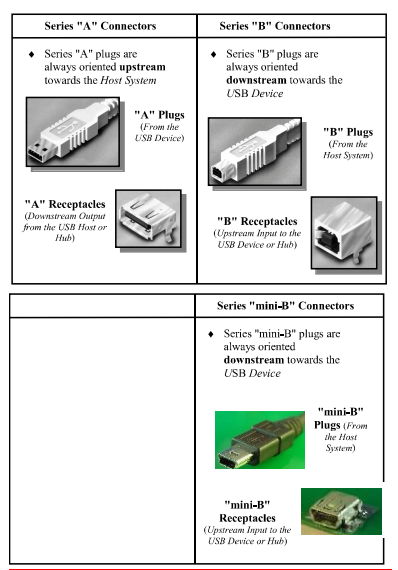
\includegraphics[scale = 0.6]{6.png}
   \caption{Tipos de conectores USB \cite{usb}}
   \label{fig:usb}
 \end{figure}
 
\end{enumerate}


\begin{thebibliography}{1}

\bibitem{serialbook}
Axelson, Jan. Serial Port Complete: The Developer's Guide. Lakeview Research LLC, 2007.

\bibitem{serialstandars}
Nestor Gabriel Forero Saboya, ``Serial Communication Standards: RS-232, RS-422 y RS-485'', (2012).

\bibitem{rs232}
Buchanan W. (1998) ``RS-232''. In: Mastering Pascal and Delphi Programming. Macmillan Master Series. Palgrave, London

\bibitem{parallelbook}
Axelson, Jan. ``Parallel port complete.'' Lakeview Research (1996).

\bibitem{IEEEparallel}
Lava Computer MFG Inc., ``IEEE 1284: Parallel Ports'', (2002).

\bibitem{usb}
Specification, Universal Serial Bus. ``Revision 2.0.'' (2000).

\end{thebibliography}


\end{document}

